\section{Keypoint extraction and matching}
\label{matching}
The first step in making a 3D reconstruction is to extract feature points from the two images.
Feature points are points of interest in an image and there are multiple ways of extracting them from an image.
A good feature points extracted from a descriptors should be repeatable, unique and consistent for all images;
occupies a relatively small area of the image (for robust to clutter and occlusion); and has a compact representation.
For example one could use dense sampling \cite{DSIFT} or random sampling,
however both these method did not prove to be useful when used in conjunction with the descriptors that we use for these keypoints.
In this report we will use the SIFT feature descriptors, introduced by Lowe\cite{SIFT} in 2004, as it has been the de facto representation method for feature points for the past years.

SIFT can robustly identify objects even among clutter and under partial occlusion, because it is invariant to uniform scaling, orientation, and partially invariant to illumination changes and affine distorting up to 60 degrees out of plane rotation.
To find keypoints SIFT uses Scale-space Extrema Detection.
It is a method to find points using the Differences of Gaussians (DoG) in a scale dependent way, to only find points that have the highest DoG in the area, which, after some refinement it can use as keypoints.
Around these keypoints a $16x16$ area is taken, which is then divided into $4x4$ subblocks.
Inside these subblocks a 8 bin orientation histogram is taken, so a 128 length feature vector is created as a representation of a keypoint.
Keypoints SIFT detect the unique corners in the image, therefore we need to have a source image with enough texture in order to have enough number of feature points.

We use a Brute Force matcher to match SIFT descriptors between images. 
For every keypoint in the first image we will find the keypoints with the smallest and the next-to-smallest euclidian distance in the second image. 
To filter out ambiguous matches we applied a ratio test. 
If the distance of the best match was bigger then a ratio of the second-to-best match then the keypoints were discarded.
By doing this ratio test reduction, we can remove keypoints that are not relevant for matching.

\begin{figure}[!ht]
	\centering
	\subfloat[Left bus image]{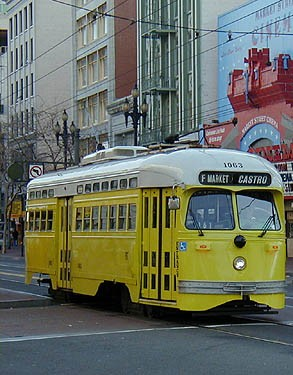
\includegraphics[width=.4\textwidth]{bus_left}} \quad
	\subfloat[Right bus image]{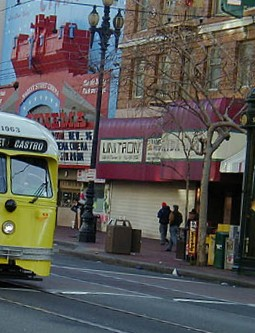
\includegraphics[width=.4\textwidth]{bus_right}}\\
	\subfloat[Matches between the images]{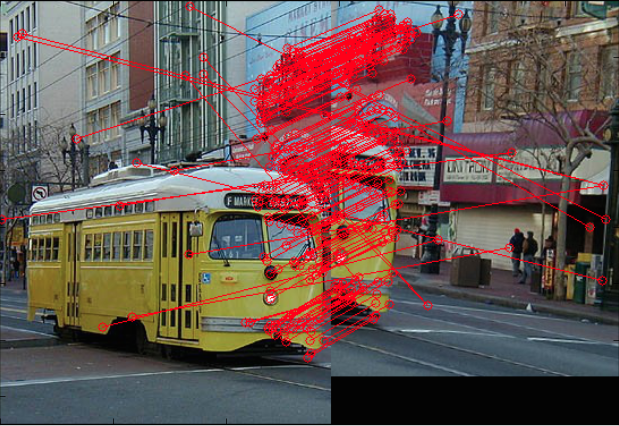
\includegraphics[width=.4\textwidth]{bus_matches}} \quad
	\subfloat[The two bus images stitched together]{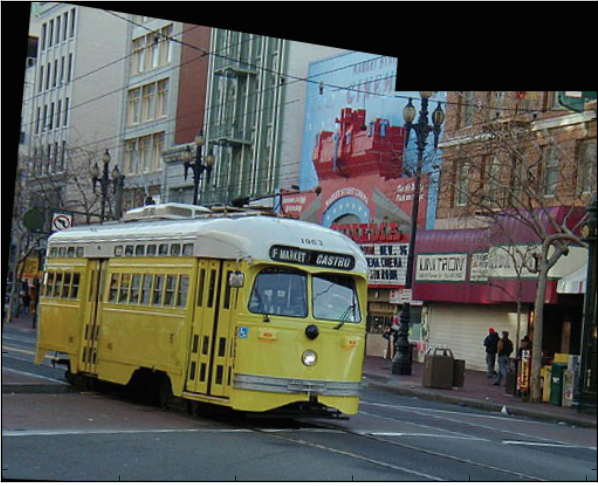
\includegraphics[width=.4\textwidth]{bus_stitched}}
	\caption{The red lines between the images are the matches that are found.}
	\label{fig:bus}
\end{figure}

After we have a good set of feature points representation, we can then estimate a homography matrix using RANSAC \cite{RANSAC}. 
In this report we implemented the improved version of RANSAC, namely Locally Optimized RANSAC (LO-RANSAC) \cite{LORANSAC}.
For the matching model, we used projection transformation matrix to make it robust to the images that were taken from different angles and distances.
We use this projection transformation because we assume that the camera point is not changed, therefore there is a homography between two views.

\begin{figure}[ht]
	\centering
	\includegraphics[width=.45\textwidth]{teddybear}
	\caption{The first image of the teddy bear dataset}
	\label{fig:bear}
\end{figure}

To test the correctness of our RANSAC implementation, we transform one of the two images using homography matrix and then draw the matched line.
With this evaluation, we can estimate an optimal number of iterations needed to compute a good homography.

\fixme{add general pipeline picture}

An example of the matching is seen in Figure~\ref{fig:bus}. 
Here we used SIFT matching, The Brute force matcher and the ratio test to get the red matches in Figure~\ref{fig:bus}a. 
They can be used to find a transform that will have the last images as the result if the image are combined after transforming.
The ratio test trimmed down the matches from 1419 matches to only 200 relevant ones, for a ratio of $.5$.
We found after some experiments that this value however does not work as well for teddy bear data (seen in Figure~\ref{fig:bear} set that we will try to reconstruct,
too many points get removed to still be able to reconstruct the teddy bear,
so we decided to have a ratio of $.75$ there.
Implementation of LO-RANSAC greatly reduce the calculation time.
With LO-RANSAC, 50 iterations is enough while with standard RANSAC we need at least 500 iterations to find a good estimation of homography
We also found out that by blurring the image with gaussian blur before extracting the feature can make the SIFT descriptor robust to background noise.
